% This must be in the first 5 lines to tell arXiv to use pdfLaTeX, which is strongly recommended.
\pdfoutput=1
% In particular, the hyperref package requires pdfLaTeX in order to break URLs across lines.

\documentclass[11pt]{article}

% Remove the "review" option to generate the final version.
\usepackage[review]{ACL2023}

% Standard package includes
\usepackage{times}
\usepackage{latexsym}

% For proper rendering and hyphenation of words containing Latin characters (including in bib files)
\usepackage[T1]{fontenc}
% For Vietnamese characters
% \usepackage[T5]{fontenc}
% See https://www.latex-project.org/help/documentation/encguide.pdf for other character sets

% This assumes your files are encoded as UTF8
\usepackage[utf8]{inputenc}

% This is not strictly necessary, and may be commented out.
% However, it will improve the layout of the manuscript,
% and will typically save some space.
\usepackage{microtype}

% This is also not strictly necessary, and may be commented out.
% However, it will improve the aesthetics of text in
% the typewriter font.
\usepackage{inconsolata}

% to gain access to images
\usepackage{graphicx}

\usepackage{booktabs}
\usepackage{tabularx}



% If the title and author information does not fit in the area allocated, uncomment the following
%
%\setlength\titlebox{<dim>}
%
% and set <dim> to something 5cm or larger.

\title{Deep Learning and Transformer-based Approaches to Sentence Level Emotion Classification}

% Author information can be set in various styles:
% For several authors from the same institution:
% \author{Author 1 \and ... \and Author n \\
%         Address line \\ ... \\ Address line}
% if the names do not fit well on one line use
%         Author 1 \\ {\bf Author 2} \\ ... \\ {\bf Author n} \\
% For authors from different institutions:
% \author{Author 1 \\ Address line \\  ... \\ Address line
%         \And  ... \And
%         Author n \\ Address line \\ ... \\ Address line}
% To start a seperate ``row'' of authors use \AND, as in
% \author{Author 1 \\ Address line \\  ... \\ Address line
%         \AND
%         Author 2 \\ Address line \\ ... \\ Address line \And
%         Author 3 \\ Address line \\ ... \\ Address line}

% \author{First Name \\
%   Affiliation / Address line 1 \\
%   Affiliation / Address line 2 \\
%   Affiliation / Address line 3 \\
%   \texttt{email@domain} \\\And
%   Second Author \\
%   Affiliation / Address line 1 \\
%   Affiliation / Address line 2 \\
%   Affiliation / Address line 3 \\
%   \texttt{email@domain} \\}



\begin{document}
\maketitle
\begin{abstract}
We evaluate three different model types on their ability to detect if Anger, Fear, Joy, Sadness, and Surprise are present in a sentence. We specifically test a neural network, the machine learning methods Binary Relevance and Classifier Chains, and the BERT-based transformer models DeBERTa and DistilBERT. Transformer models received the highest micro F1 scores, with DeBERTa and DistilBERT roughly tied in performance. 

\end{abstract}

\section{Introduction}

Understanding emotions expressed in text is crucial for improving human-computer interaction and minimizing miscommunication in text-based communication. This study focuses on the multi-label classification of sentence-level text into five key emotions: Anger, Fear, Joy, Sadness, and Surprise, as originally framed in SemEval 2025 Task 11: Bridging the Gap in Text-Based Emotion Detection. The specific task goal is “Determining what emotion most people will think the speaker may be feeling given a sentence or a short text snippet uttered by the speaker.” Leveraging datasets provided by SemEval, we evaluate the performance of transformer-based models, including DeBERTa and DistilBERT, alongside traditional machine learning methods such as Classifier Chains and Binary Relevance.We also build upon the SemEval-provided baseline, a basic neural network, introducing optimizations that significantly enhance recall and F1 scores. 

To match the original metric used by the SemEval baseline model we will be using F1 scores as our primary metric for measuring model performance. To examine cross-linguistic performance, we extend our analysis to Amharic text, translated into English via the Google Translate API, revealing notable performance differences due to translation and label reliability issues. Hyperparameter tuning through grid search further refined model performance, yielding substantial improvements.


\section{Related Works}

Multi-label emotion classification has gained significant attention due to the inherent complexity and the various use cases such as healthcare and wellbeing as well as author intention analysis. Multi-label classification has the capability of detecting and expressing the larger complexities of a given sentence audio, or even an image that a single label can’t capture. The work from “SemEval 2018 Task 1: Affect Tweets” has been a cornerstone for this field, offering annotated tweets with a range of affective dimensions, including basic emotions like joy, sadness, and fear, and intensity measures for valence, arousal, and dominance \cite{mohammad-kiritchenko-2018-understanding}. These annotations enable models to predict the co-occurrence of multiple emotions and their varying intensities, addressing a key challenge in emotion recognition. Innovations like SpanEmo have further advanced this field by reframing multi-label emotion classification as a span-prediction problem, allowing for the identification of emotion-specific phrases in a sentence \cite{alhuzali-ananiadou-2021-spanemo}. Such approaches have improved the ability to capture overlapping emotions and learn meaningful associations between words and emotion classes, resulting in stronger model performance across multiple datasets.

Although we were not able to find extensive research on multi-label Amharic emotion classification, cross-language emotion classification has entered the realm of multi-label emotion detection, particularly through the exploration of code-mixed and multilingual corpora. For example, datasets combining English and Roman Urdu have addressed the unique challenges of detecting emotions in mixed-language contexts. The application of state-of-the-art deep learning techniques, such as BERT and XLNet, alongside traditional machine learning methods, demonstrated the efficacy of both paradigms for these tasks. Additionally, Virtual Adversarial Training (VAT)  has shown promise in leveraging unlabelled data to improve multi-label classification performance across languages such as Arabic, Spanish, and English.\cite{gupta-2021-multilingual} By building on multilingual datasets from the SemEval competition, VAT-based methods revealed the benefits of semi-supervised learning in achieving robust cross-lingual emotion recognition.

Building on these advancements, our work seeks to improve multi-label emotion classification particularly by using available transformer models and optimizing them, and by addressing the challenges identified in prior studies, including co-occurring emotions and nuanced contextual relationships. Inspired by the methodologies explored in the SemEval 2018 Task 1 and subsequent research, we aim to achieve state-of-the-art F1 for our specific dataset using DistilBERT and DeBERTa. This approach enables us to enhance emotion detection for both fine-grained and overlapping categories, leveraging insights from prior innovations to bridge gaps in current models and datasets.





\section{Dataset}

We used four datasets during our research: one to guide training and three to benchmark performance.

\subsection{Training Dataset}
Our English training dataset consists of 2768 sentences with emotion labels. An example can be seen in Figure 1:

\begin{figure}
    \centering
    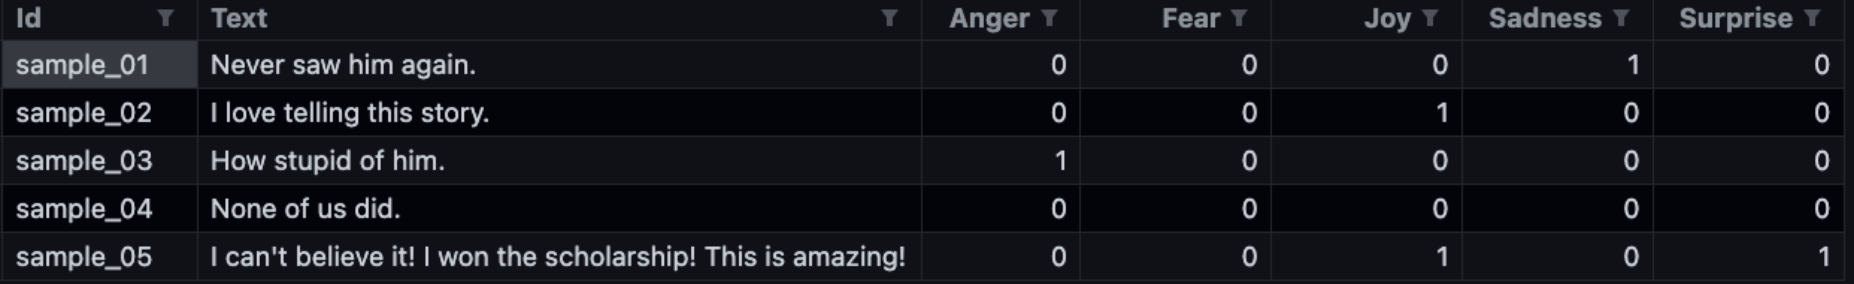
\includegraphics[width=\columnwidth]{dataset_preview}
    \caption{\textit{Example rows in training dataset.}}
\end{figure}

This dataset was provided by the SemEval organizers. We do not know where their examples are sourced from as the organizers have not yet published a paper detailing their data collection methods. However, the CodaBench online evaluator refers to the examples as tweets. This leads us to believe the examples were sourced from X. 

The largest issue we faced was class imbalance in the dataset. Specifically, the Fear label shows up significantly more frequently than all other labels, as seen in Figure 2.

\begin{figure}
    \centering
    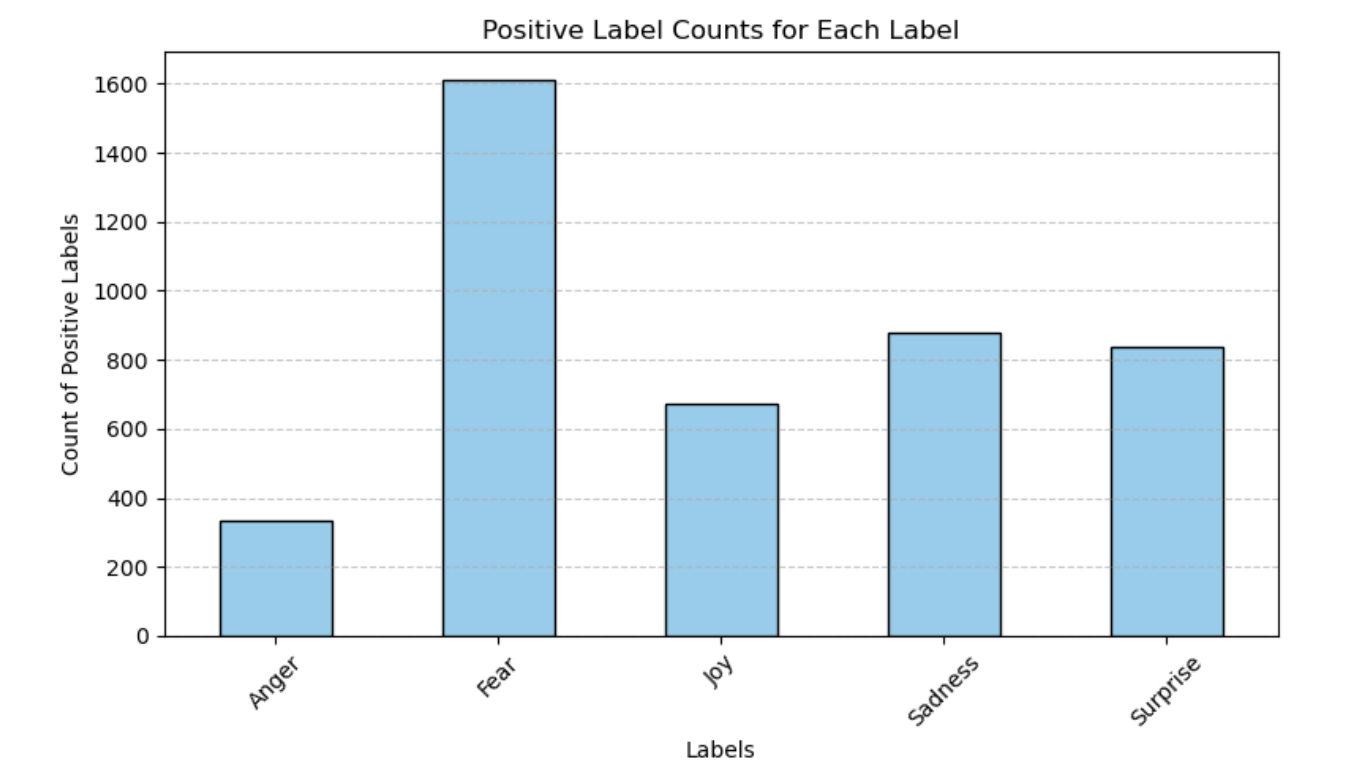
\includegraphics[width=\columnwidth]{train_labels.png}
    \caption{\textit{Label distribution in English training set. Total label count is larger than length of the dataset because of the multi-label nature of the data.}}
\end{figure}

We experimented with adding class weights to help re-balance which will be discussed further in the Results section.

We also had concerns with the validity of emotion labels – in some cases the labels did not correspond to the emotions we had observed in the sentence. We chose to not modify the dataset to keep any possible error consistent across the dataset.\cite{mohammad-2023-best}

We conducted a brief self-labeling exercise to test the accuracy of the given dataset. We randomly selected a sample of 30 sentences from the training dataset and chose to label it ourselves. When comparing our self-made labels with the annotated labels, we found that many discrepancies are "reasonable" - or that the margin of error was subjective enough that a random individual could reasonably create that annotation. As a result, we decided to not modify our training dataset for the results of these experiments. In the future, we may further explore the dataset after the SemEval organizers release more information.

\subsection{Evaluation Datasets}

We used three additional datasets to test our model’s ability to perform on unseen data – namely data from another source language and created by a non-SemEval party.

\subsubsection{Evaluation Dataset 1 - English}

The SemEval English development set consists of 116 example sentences with no emotion labels. The data is formatted the same way as the training set. To understand our model’s performance, we generated predictions on this dataset and submitted them to the SemEval Task 11 on CodaBench.

\subsubsection{Evaluation Dataset 2 - Amharic}

The SemEval Amharic training set was also provided by the task organizers and consists of 3,549 labelled English sentences. The original dataset was in Amharic, and we translated each example to English using the Google Translate API. The original dataset also included a Disgust emotion that was not in our training data, so we excluded it while cleaning. Other cleaning tasks involved rearranging the order of emotion labels to match the order in our training dataset.

\subsubsection{Evaluation Dataset 3 - Helsinki XED}

We also used the Helsinki XED dataset from the University of Helsinki. We sourced this dataset from the HuggingFace Datasets repository. This dataset contains 12,244 sentences with the same labels as our training dataset (after removing Anticipation, Surprise, and Trust labels). The sentences were sourced from the OPUS corpus of English movie subtitles and were mainly annotated by university students learning about sentiment analysis \cite{ohman-etal-2020-xed}.


\section{Methods}

The task of multi-label emotion classification involves predicting the presence or absence of multiple emotions within a given text. This task can be approached in two distinct ways: as a holistic multi-label classification problem or as a series of single-label classification tasks performed independently. In the holistic approach, the model simultaneously predicts all the emotion labels, capturing interdependencies and correlations between emotions. Conversely, the single-label approach treats each emotion as a binary classification task, predicting the presence or absence of one label at a time. Both approaches have their merits and challenges—while the holistic method benefits from learning relationships between emotions, it requires a more complex implementation, and the single-label method, though simpler, risks overlooking nuanced interdependencies and may be computational intensive if we train a model for each separate emotion. 

\subsection{Enhancing the Baseline Neural Network}

To begin tackling the multi-label emotion classification task, we built upon the baseline neural network by introducing additional layers and fine-tuning the architecture. The baseline model comprised a single hidden layer with 100 units, followed by ReLU activation and a dropout layer. While straightforward, this architecture was limited in its ability to learn complex patterns within the dataset.
Our enhanced model introduced two hidden layers, each with 128 and 64 units respectively. Between these layers, we employed ReLU activations to capture non-linear relationships in the input data. Additionally, batch normalization was integrated to stabilize training and improve convergence, and dropout layers with a probability of 0.3 were used to avoid overfitting. The multi-layer architecture aimed to provide the model with a deeper capacity to learn intricate interactions between features and emotion labels, which are crucial in a task like emotion classification.

To further boost F1 scores, we lowered the classification threshold to 0.37, enabling the model to capture more true positives and significantly improve recall. This adjustment was particularly effective for rare emotion labels, which might otherwise be overlooked with a standard threshold. By balancing model complexity and with threshold selection, our enhanced neural network demonstrated an improvement in F1 score compared to the baseline, underscoring the value of architecture tweaks in multi-label emotion classification.

\subsection{Exploring Traditional Multi-Label Classification Approaches}

To further improve performance on the task, we experimented with traditional machine learning approaches using the sklearn python library, specifically Binary Relevance and Classifier Chains. These models were implemented using Logistic Regression (LR), Random Forest (RF), and Support Vector Machines (SVMs), with hyperparameters tuned via grid search \cite{zhang2018binary}. Binary Relevance treated each label as an independent binary classification problem, while Classifier Chains modeled dependencies between labels by sequentially training classifiers, each incorporating predictions from previous labels. Both methods were trained on 95\% of the eng\_train.csv dataset provided by SemEval, with the remaining 5\% used as a local development set for evaluation.

Although these model adjustments yielded models that outperformed the baseline neural network in terms of precision, they had lower Macro F1 scores by about 3 percentage points. Additionally, these models, particularly SVM based versions, required significant training time, showing the need for more computationally efficient methods of large-scale multi-label classification.

\subsection{Transformer Model Fine-Tuning: DeBERTa and DistilBERT}

After exploring traditional machine learning models and neural networks, we shifted our focus to fine-tuning transformer models to solve the task. We specifically experimented with DeBERTa \cite{he2020deberta} and DistilBERT \cite{sanh2019distilbert}, both of which demonstrated superior performance compared to non-transformers models. These models, pre-trained on large corpora, have the advantage of understanding contextual relationships and word placements better, which is why they are particularly effective for nuanced language tasks like emotion detection. 

We chose these models carefully: we hypothesized DeBERTa would be stronger at attending to the context and interdependencies of words more efficiently, and we were curious if DistilBERT's reduced size would lead to performance drops.

For the fine-tuning process, we initially used a class-weighted approach, which helped address the issue of label imbalance in the training data. Many emotions in the SemEval dataset are infrequent, and without class weighting, the models might have biased predictions towards more frequent labels. By assigning higher weights to underrepresented classes, we ensured that the models would give more attention to rare labels during training, which improved the model’s ability to detect emotions like anger. However, the increase we saw in performance was relatively small, increasing our F1 score by only 0.2 percentage points. After debate, we chose to stop using class weights so that our model is not too biased towards the label distribution of one particular dataset, especially as we apply the model to various other datasets that have a different distributions of classes than our training dataset. As we collect more data and understand the relationship between the labels more clearly, we may reinstate more effective and accurate class weights.

We fine-tuned both DeBERTa and DistilBERT using a grid search over learning rate and batch size \cite{WU201926}. The learning rates were tested at values of [2e-4, 2e-5, 2e-6], while the batch sizes were varied between [8, 16, 32]. The model was optimized using a binary cross-entropy loss function and a sigmoid activation for each label, allowing it to predict the probability of multiple emotions for a single input text. This configuration is well-suited for multi-label classification as it treats each label independently and assigns a probability score for each. The ability to fine-tune these pre-trained models allowed us to capture subtle contextual meanings in the text, significantly improving the classification of co-existing emotions. The model consistently performed best on a learning rate of [2e-5] and with a batch size of [8] for both DeBERTA and DistilBERT. We proceed with this model for our official tests.  

Between DeBERTa and DistilBERT, we observed that DistilBERT, the smaller version of BERT, delivered marginally best results. Despite its reduced size, DistilBERT managed to maintain better performance while being more computationally efficient. This made it an ideal candidate for further experimentation, as it balanced performance and efficiency. By leveraging  transformer models and fine-tuning them with optimal hyperparameters, we achieved our highest classification F1 scores. This solidified our decision to pursue transformers as the primary models for solving the multi-label emotion classification task.

\section{Results}

To improve our F1 score against the baseline, we conducted a number of experiments. We first extended the baseline neural network provided. We then tested an assortment of machine learning frameworks. After seeing minimal increases in performance, we evaluated performance using DeBERTa and DistilBERT.

\subsection{Baseline}

The SemEval task organizers provided a baseline to use in the competition. Their model consisted of a 2-layer neural network that was trained on the English dev dataset. Their threshold was 45\%. The organizers tested their model with and without class weights. The results are summarized in Figure 3. 


\begin{figure}
    \centering
    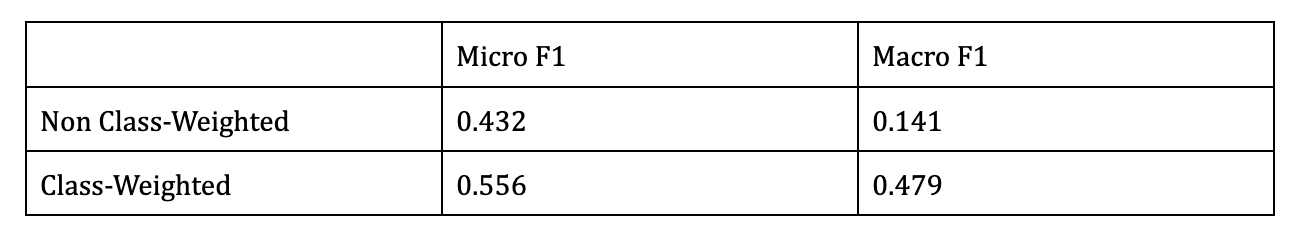
\includegraphics[width=\columnwidth]{baseline}
    \caption{\textit{Baseline F1 scores.}}
\end{figure}


We assume baselines of Micro F1 = 0.556 and Macro F1 = 0.479.

\subsection{Experiment 1 – Deep Learning}

To create an extended neural network, we added two hidden layers along with RELU and batch normalization layers to the baseline model and decreased the probability threshold of predicting a positive label to 0.37 to help us with the recall. These changes resulted in a micro F1 score of 0.606 and a macro F1 score of 0.558. These are above our baseline scores by 5\% and 7.9\% respectively.

\subsection{Experiment 2 – Machine Learning}

We test two types of machine learning model types: Binary Relevance and Classification Chain. In each model, we tested further across Logistic Regression, Random Forest, and SVM algorithms. 

We found that SVMs resulted in the highest F1 scores. The results can be seen in Figure 4:

\begin{figure}
    \centering
    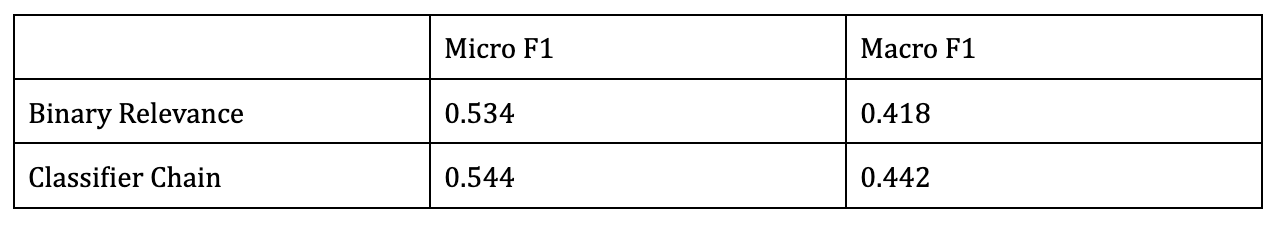
\includegraphics[width=\columnwidth]{exp_2_results}
    \caption{\textit{SVM experiment results.}}
\end{figure}

The most precise model type (Classifier Chain) performed 1.2\% worse (micro) and 3.7\% worse (macro) than our baseline.


\subsection{Experiment 3 – Transformers}

We also tested two distinct BERT models: DistilBERT and DeBERTa.

\subsubsection{DistilBERT Hyperparameter Training}

Baselines for the transformer models were derived by choosing 60\% of the training set and further dividing the subset into a 95/5 train-test split. 
With HuggingFace’s default TrainingArgument and Trainer parameters, the model scored a micro F1 of 0.68 with a threshold of 0.4. With the addition of class weights, the model scored a micro F1 of 0.682 with a threshold of 0.55. We chose to not continue with class weights as we reasoned that not all datasets will contain the same class imbalance as this subset of data. Our baseline from these experiments was a micro F1 score of 0.68.

We then performed a grid search over batch size and learning rate, testing thresholds between 0.35 and 0.65 for all parameter combinations. The results can be seen in Figure 5:

\begin{figure}
    \centering
    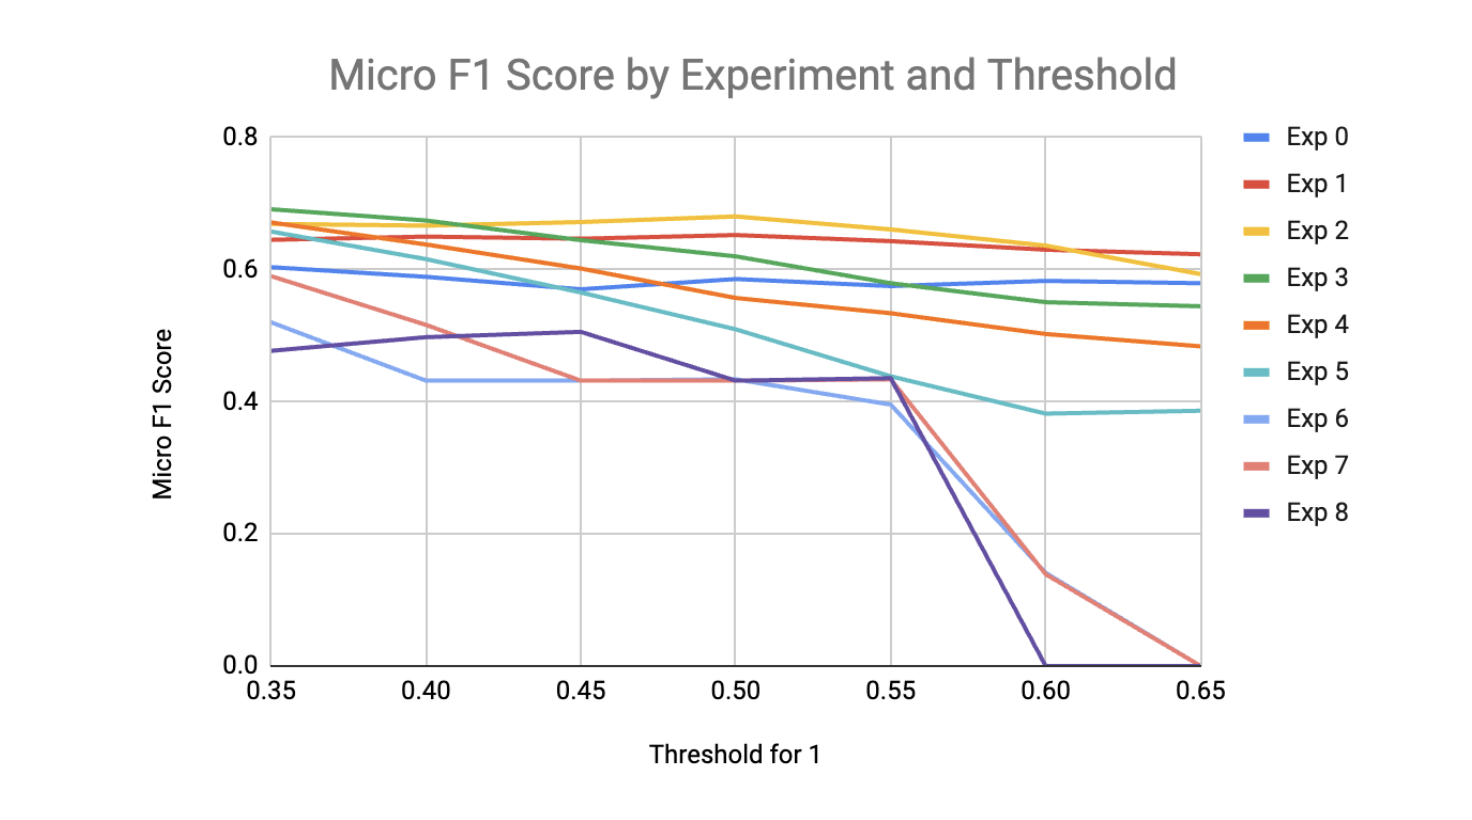
\includegraphics[width=\columnwidth]{distil_testing}
    \caption{\textit{DistilBERT grid search. Exp 0 – Exp 8 refer to individual combinations of batch size and learning rate}}
\end{figure}

Nearly all experiments decreased performance. The best hyperparameter combination was Learning Rate = 2e-5, Batch Size = 8, and threshold = 0.35. This combination scored a Micro F1 score of .691, or a 1.1\% increase over the DistilBERT baseline. This DistilBERT hyperparameter combination performed the best out of all experiments on the miniature training set.


\subsubsection{DeBERTa Hyperparameter Training}

DeBERTa experiments used the same 60\% dataset, split into 95/5 train-test split as DistilBERT.  

With HuggingFace’s default TrainingArgument and Trainer parameters, the model scored a micro F1 of 0.67 with a threshold of 0.4. We then performed the same grid search over batch size and learning rate, testing thresholds between 0.35 and 0.5. The results can be seen in Figure 6.

\begin{figure}
    \centering
    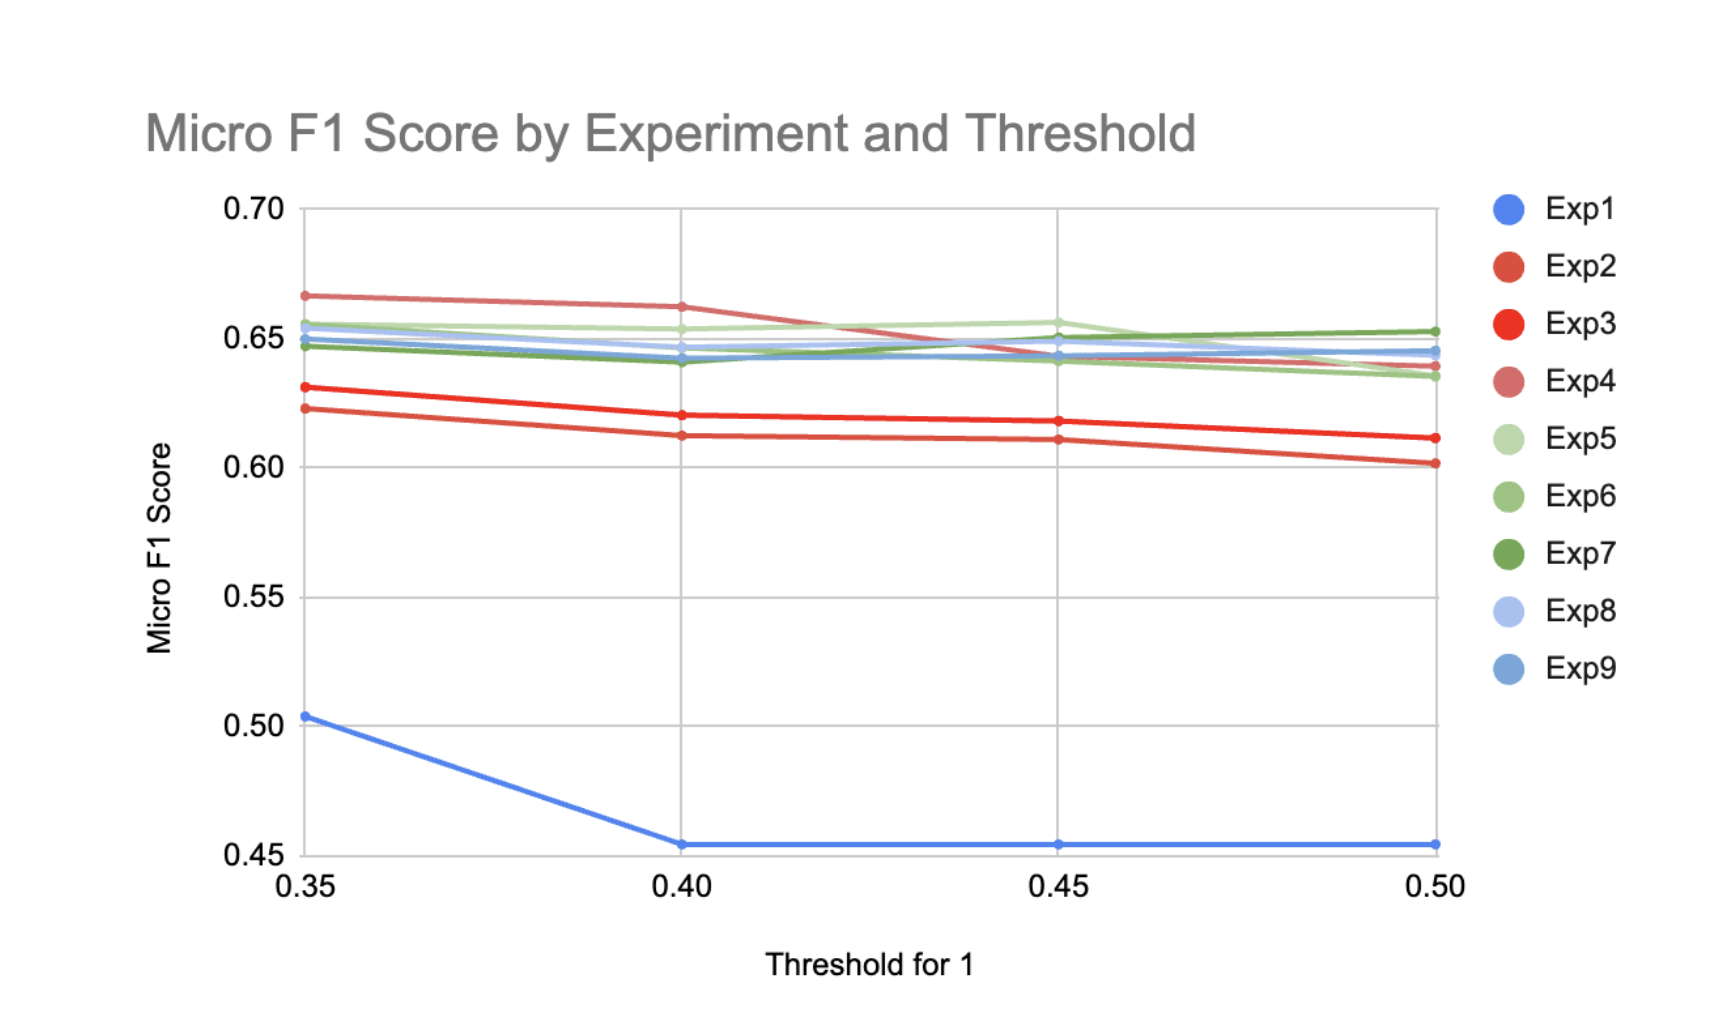
\includegraphics[width=\columnwidth]{debert_testing}
    \caption{\textit{DeBERTa grid search. Exp 1 – Exp 9 refer to individual combinations of batch size and learning rate}}
\end{figure}

Nearly all experiments decreased performance again. The best hyperparameter combination was Learning Rate = 2e-5, Batch Size = 8, and threshold = 0.35 as well. This combination scored a Micro F1 score of .681, or a 1.1\% increase over the DeBERTa baseline. To better understand why this model was weaker is, we calculated micro Precision and Recall: the model scored 0.62 on Precision and 0.7 on Recall. This suggests that the model struggled with over-identifying certain emotions. 

\subsubsection{Evaluation on Dev Set}

After identifying the best hyperparameters, we trained an instance of each model on the full English training set. To understand how well our model generalizes to unseen data, we evaluate on the dev set eng\_a.csv. To do this, we created a CSV with our dev set predictions and submitted it to CodaBench, the official submission site for the SemEval task. After submitting our CSV results, we received micro and macro F1 scores.  

On the dev set, the DistilBERT model received a micro F1 score of 0.715 and a macro F1 score of 0.712. The DeBERTa model received a micro F1 score of 0.715 and a macro F1 score of 0.71.

We believe the increase comes from the fact the model was trained on the entire English training set (instead of 60\%) and the dev set is similar to the training set in sourcing and annotation method.


\subsubsection{Evaluation on a Non-English Dataset}

To better understand the effect of translating a dataset on emotion classification, we evaluate our model’s predictions on the entire SemEval Amharic training dataset (that we translated into English). 

On this dataset, the DistilBERT model received a micro F1 score of 0.366 and a macro F1 score of 0.359. The DeBERTa model received a micro F1 score of 0.378 and a macro F1 score of 0.362.

We believe the performance drop can be attributed to somewhat unreliable annotations in the original dataset and Google Translate skewing the meaning of sentences. 

Although the data source was not revealed, the content of the Amharic dataset seemed to have been sourced from social media posts and responses to these posts. We are suspicious of the labeling since the majority of the examples seem to have only one positive label. Considering this, we might have created an unintended bias in the dataset by removing the disgust column which possibly resulted in rows with no labels. In regards to the quality of the translation, we entirely depended on the Google Translate API, which worked well with translating individual words, but severely underperformed in translating the contextual meaning or the figurative language used. This resulted in some translated examples that did not portray the same emotion in English as they originally did in Amharic.


\subsubsection{Evaluation on a Third-Party Dataset}

To study our model’s ability to generalize on data not created by SemEval, we evaluate its predictions on the entire Helsinki XED English dataset.

On this dataset, the DistilBERT model received a micro F1 score of 0.501 and a macro F1 score of 0.512. The DeBERTa model received a micro F1 score of 0.487 and a macro F1 score of 0.498.

We believe the stronger performance on this dataset compared to the Amharic dataset is due to the fact that this dataset was created in English. However, performance was weaker than on the dev set because it was annotated and sourced by a different group who likely encoded different judgment metrics into their ratings.


\subsection{All Results}

Figure 7 displays an overview of all experiments and corresponding results.

\begin{figure*}
    \centering
    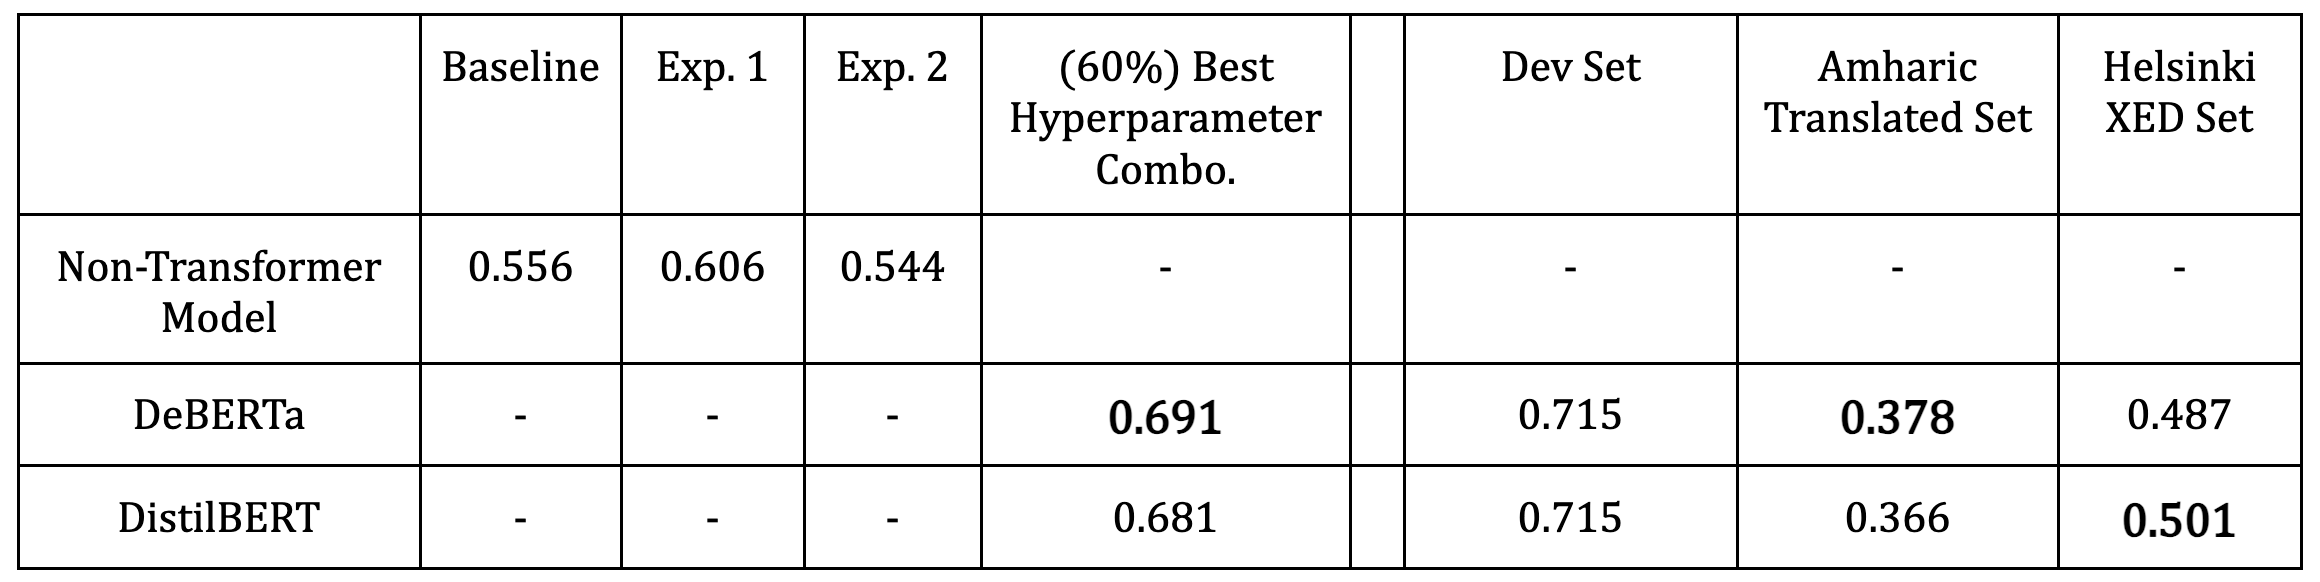
\includegraphics[width=\textwidth]{results_table_2}
    \caption{\textit{Final micro F1 results. The right half of the table corresponds to evaluation results.}}
\end{figure*}

\section{Ethics and Limitations}

\subsection{Ethical Considerations}

These breakthroughs are exciting, but it is crucial to consider ethical risks of emotion classification technology. Specifically, emotions are expressed differently in different cultures (i.e. use of dialect-specific terms or modes of communication), so it is crucial that models are trained on sentences from vastly different origins. Similarly, if a model disproportionately associates sentences from a certain racial or ethnic group with a certain emotion (i.e. anger), it could potentially propagate harmful stereotypes. It is crucial that developers ensure their models are not biased against specific populations while simultaneously ensuring protection for users who created the data.

\subsection{Limitations}

Our work is limited by the amount of experiments we performed at each stage of the research process. We could have tested more BERT models (such as ALBERT and RoBERTa), experimented with different hyperparameters (such as momentum or the number of training epochs), or test on other translated texts and datasets. As a result, our findings are only generalizable to two specific models (DistilBERT and DeBERTa) and one non-English language (Amharic). Additionally, we only trained and tested models to handle text in English. Our algorithm was slightly naive: if time permitted we would have experimented with different thresholds for each emotion. Additionally, our datasets did not have any metric that validated their legitimacy. Although we did a self-labeling exercise and decided that the dataset we have is a reasonable annotation by a random individual, we have no basis for arguing that this dataset could be generalizable. The nature of emotion classification leaves a lot of room for error. Specifically because we are attempting to classify perceived emotions, we will struggle to find a general "perception" of emotions.

\section*{Conclusion}
We tested a variety of models on the given SemEval dataset, ranging from neural networks and Support Vector Machines to transformers, and concluded that transformers are the strongest model to conduct multi-label classification. From there, we performed a variety of tests to fine-tune our model’s parameters to achieve our highest F1 score, eventually selecting a learning rate of [2e-5] and a batch size of [8] for our model. We trained our model on the full eng.csv dataset from SemEval Task 11 Track A and applied it to 3 datasets: the dev set, a translated Amharic dataset, and the Helsinki XED dataset. Our results varied heavily - ranging from a 0.377 F1 score on the translated Amharic set to a 0.715 F1 Score on our SemEval dev set. In between, we received a 0.501 F1 Score on the third party Helsinki dataset and a 0.67 F1 Score on our SemEval training set.

Noticeably, our F1 scores from the English SemEval datasets - both dev and training - were higher than our scores for the remaining datasets. This can be attributed to the fact that these datasets were the most similar to our training set - matching the language and the source (SemEval). Comparatively, however, we can see that the model’s performance on the translated Amharic is worse than on the Helsinki set. We theorize that translating a language to English does not correctly catch all of the cultural phrases and contexts. Translation resulted in a large penalty in our F1 score, as detecting emotion heavily relies on interpreting context and phrases correctly. Regardless, our models were not able to generalize well, as they achieved a F1 score of 0.512 on the Helsinki dataset (which was in the same source language as the SemEval datasets). We believe that the drop-off between the Helinski and SemEval dataset results could be attributed to the content of the sentences and the subjectivity of the labels. SemEval’s dataset is mostly random, short sentences that had no focus or consistency between each other. On the other hand, the Helsinki dataset had many repeated words, with many example starting with the same phrase. In addition, the datasets were annotated by different individuals. Thus, we conclude that the variations between our training dataset and the Helsinki dataset resulted in large penalties for our F1 score, though not as large as the penalties from translating a different language.

Our immediate next step would be to focus on reshaping our datasets by integrating class weights. We found that a core aspect of multi-label emotion recognition is the correlation between different emotions. For example, we observed that “Fear” appears frequently with “Sadness” or with “Surprise” in our SemEval training set. We have determined that this results in certain emotions appearing far more frequently than others, especially depending on the presence of a linked emotion. To start this process, we would relabel a larger portion of the dataset ourselves to  confirm this correlation. Based on the results of our relabeling, we look to implement fine-tuned class weights to our training dataset and test the newly established model onto all previous datasets. We predict that with robust class weights, our model will be more generalizable to different datasets.


% Entries for the entire Anthology, followed by custom entries
\nocite{yu2018improving}
\bibliography{custom}
\bibliographystyle{acl_natbib}

\appendix

\section{Code Link}

GitHub: \url{https://github.com/Henok-foslyk/NLP\_InsideOut}

\end{document}
